\chapter{File Formats}
In the following section, I will use stdint.h style names for naming datatypes with exact bit width.

\section{PAL files}
    PAL files are colour pallettes used by the image formats in diablo. They always contain 256 colours, and each colour is 3 bytes long (r, g, and b bytes), so they are always 768 bytes long. Image files refer to them by index into the file (so, a two would represent the 3rd colour, or the third group of three bytes).

\section{CEL image files}
	CEL image files use the CEL and CL2 file extensions. There are some minor differences between the two, but they are fundamentally the same. The basic capabilities of the format are run length encoding, and transparency (but only total transparency, not partial). Each file can contain multiple frames that can represent parts of an object, frames in an animation, or even tilesets for levels.

	\subsection{File Header}
	\label{sec:fileheaders}
	The file header is composed of a series of uint32\_t. The first is the number of frames. This is followed by an offset from the start of the file for each frame, and finally, an offset to the end of the file. Illustrated below is a pseudo-C struct representing it's structure.
	\begin{lstlisting}
struct fileHeader
{
	uint32_t numFrames;
	uint32_t frameOffsets[numFrames];
	uint32_t endOffset;
};
	\end{lstlisting}
	 This header is common to both CEL and CL2 files.
	 
	\subsection{Frame Headers}
	\label{sec:frameheaders}
	Some CEL frames contain headers at the start of the frame. It is 5 uint16\_t (10 bytes) long. Entries appear to be pointers to positions in the file, which when reached during decoding will leave us with a specific number of lines created, but I only understand the second entry (and it is the only one of use to us). This entry gives us a position in the file, that when we reach it, we will have processed 32 lines of pixels in the image. By checking how many pixels have been genrated by the time we get to that point, we can divide this number by 32 to get the image width.
	The first entry is always 10, as it points to the start of the image data.
	The third entry may point to the end of the 64th line (if it exists) and so on, but I have not investigated this as it is of no use to me.
	
	\subsection{CEL Frames}
	There are two kinds of plain CEL frame. One is the "normal" kind, which contains animations of objects. Examples of these can be found in the items directory in DIABDAT.MPQ. The other is tileset cel frames. As the name implies, these contain the tilesets for levels. These are found only in levels/*/*.cel.
	A given CEL file will only conatin one of these types, not both.
A colour in a CEL frame will always be a single byte index into a palette.

	\subsubsection{Normal CEL Frames}
	Normal Frames are composed of a series of command and data blocks.
	Each block is a uint8\_t.
	The command blocks contain instructions about what to do next during decoding. The data blocks contain indices into a palette to obtain a colour value.
	
	Decoding is performed by starting at the start of the file (the first block will always be a control block), and executing the command there. 
	\\Then you advance by the number of blocks specified by the current block, which brings you to the next control block, and so on until you have decoded the entire frame. There are two kinds of control block: Regular and Transparency.
	
	\emph{Regular blocks} are denoted by values $\leq 127$. When you encounter a regular block, it's value indicates how many pixels it contains. For example, if you encounter a Regular block with value 10, the next 10 blocks are data blocks, one pixel each, and the 11th block after is the next control block.
	
	\emph{Transparency blocks} are denoted by values $> 127$. When a transparency block is encountered, it indicates $256-$block value transparent pixels. Transparency blocks do no use any data blocks, and so the immediate next block is the next control block.
	
	Below is a sample implementation of decoding a frame.
	
	\begin{lstlisting}
// Frame is the raw frame from the file, pal is a palette
// raw_image is the destination for decoded pixels
void CelFile::normal_decode(vector<uint8_t>& frame, Pal pal, vector<colour>& raw_image)
{
    size_t i = 0;
    
    for(; i < frame.size(); i++)
    {   
        // Regular command
        if(frame[i] <= 127)
        {    
            size_t j;
            // Just push the number of pixels specified by the command
            for(j = 1; j < frame[i]+1 && i+j < frame.size(); j++)
            {
                int index = i+j;
                uint8_t f = frame[index];
                colour col = pal[f];
                raw_image.push_back(col);
            }
    
            i+= frame[i];
        }

        // Transparency command
        else // >= 128
        {
            // Push (256 - command value) transparent pixels
            for(size_t j = 0; j < 256-frame[i]; j++)
                raw_image.push_back(transparentColour()));
        }
    }
}
	\end{lstlisting}

\subsubsection{Tileset CEL frames}
	These CEL files have the same format as normal CEL files, but the data in the franes is different. There are a number of possible "types" of frame within tileset CEL files. All of them are always of width and height 32.
\begin{itemize}

	\item{Raw:} Raw frames are just that, 32*32=1024 bytes of raw colours, with no transparency. 
	
	\item{Normal:} Some frames are normal frames as described in the previous section. These never have headers when contained in tilese CEL files.
	
	\item{Greater/Less than frames:} These are the most interesting frame type in cel files. They are the tiny triangles which make up half of an isometric block on the map. The name greater/less than is borrowed from ProjectDDT\cite{ddt}. \\

\includegraphics{ltgt}\\ Above is an example of a less than and greater than frame respectively. As you can see, when placed together, they make up a 64*32 pixel isometric block.\\
You can tell if a frame is a less than or greater than frame by looking at the contents. A certain set of bytes will be zeroed in both cases.\\
Less Than: bytes 0,1,8,9,24,25,48,49,80,81,120,121,168,169,224,225\\
Greater Than: bytes 2,3,14,15,34,35,62,63,98,99,142,143,194,195\\

	These bytes are clearly in pairs. Each pair marks the end of two rows of colour, as shown in the image below:\\
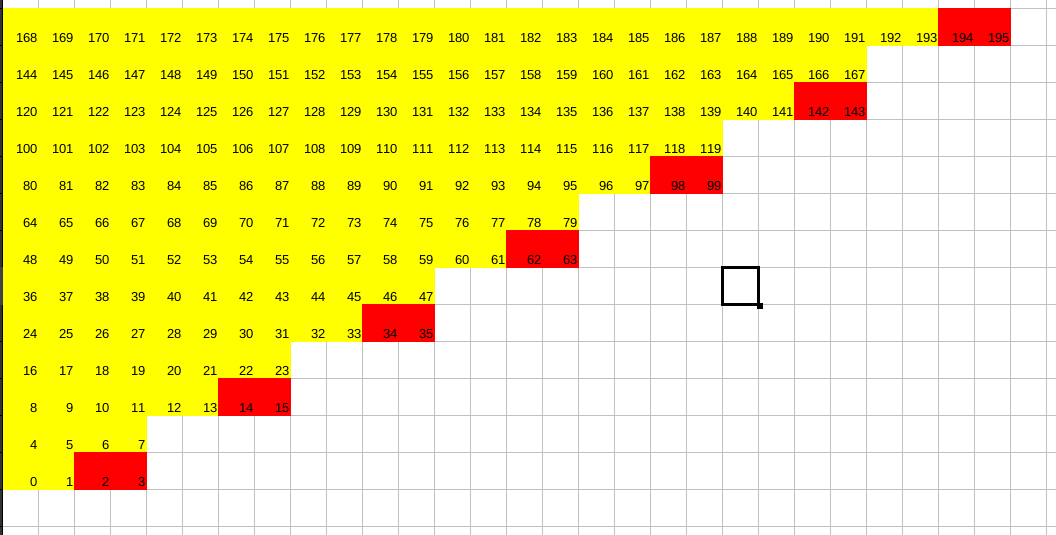
\includegraphics[scale=0.3]{ltgt-markers}\\
The yellow blocks are the bytes in between the markers, which contain colour indices, the red are the markers themselves. When rendereing, these are ignored, so all non-yellow blocks are transparent.

	For a given less/greater than frame, the first half will always conform to the scheme described above, but this only shows half the image.
	From there, there is variation. Some frames will have another half encoded the same way, with the following markers:\\
	Less Than Second Half: bytes 288,289,348,349,400,401,444,445,480,481,508,509,528,529\\
	Greater Than Second Half: bytes 245,255,318,319,374,375,422,423,462,463,494,495,518,519,534,535\\
	
	If these markers are not present, however, the second half is raw with no transparency, so we can just pull it out directly, eg:\\
	
\includegraphics[scale=0.5]{rawtop}
\end{itemize}

\newpage

\subsection{CL2 Frames}
	CL2 Frames are very similar to CEL frames, with the main difference that the use run-length encoding for colours as well as tranparency. They also always have frame headers.
   In addition to the regular and transparency blocks used in normal CEL frames, they also have RLE blocks, which indicate the number of times to repeat the colour indicated by the next block.
   Below is some C++ code that illustrates this:
   
   \begin{lstlisting}
void cl2Decode(const std::vector<uint8_t>& frame, 
   const Pal& pal, std::vector<Colour>& rawImage)
{
    size_t i = 10; // CL2 frames always have headers

    for(; i < frame.size(); i++)
    {
        // Color command
        if(frame[i] > 127)
        {
            uint8_t val = 256 - frame[i];
           
            // Regular command
            if(val <= 65)
            {
                size_t j;
                // Just push the number of pixels specified by the command
                for(j = 1; j < val+1 && i+j < frame.size(); j++)
                {
                    int index = i+j;
                    uint8_t f = frame[index];

                    Colour col = pal[f];

                    rawImage.push_back(col);
                }
              
                i+= val;
            }

            // RLE (run length encoded) Colour command
            else
            {
                for(int j = 0; j < val-65; j++)
                    rawImage.push_back(pal[frame[i+1]]);
          
                i += 1;
            }
        }
        
        // Transparency command
        else
        {
            // Push transparent pixels
            for(size_t j = 0; j < frame[i]; j++)
                rawImage.push_back(Colour(255, 0, 255, false));
        }
    }
}
   \end{lstlisting}
   
   As can be seen above, the blocks use different values, but the basic structure is the same as CEL frames.
   
 	\subsection{Frame Width}
 	Frame width determination is not as simple as it might sound. None of the frame formats have image dimensions built in, but there are a number of heuristics to find them.
 	For images with a frame header, the technique described in section \ref{sec:frameheaders} can be used. 
 	For tileset frames, the width is always 32.
 	For all others, there is another technique, which will work so long as the image width is not a multiple of 127, on images with no transparency (which headerless images seem to be).
 	
 	The maximum stretch of a Regular block is 127. A block will never straddle two lines, so if for example a frame were of width 130, there would be a series of 127 blocks followed by 3 blocks, one pair for each line.
 	
 	We can abuse this fact, by starting at the start of the frame, and adding together each command block until we find one that is not 127. At that point the sum of the previous 127s + the current block is the width of the image, as the current block has to exist to split on a line.
 	
 	\subsection{CEL Archives}
 	Some CEL and CL2 files are in fact archives of multiple CEL/CL2 files, respectively. These are used to store multiple rotations of an animation (eg walk animation in all 8 possible directions). These files have headers at the start, which consist of a number of uint32\_t s, each one pointing to a file contained in the archive.
 	
 	As there is always 8 images in such files, the first pointer will always be 32, as it will always point to the first byte after the headers, which are 8*4=32 bytes long, so it is possible to tell which files are archives by checking the first uint32\_t against 32.
 	
 	For CEL files, that's all there is to it, but for CL2, it's a little more complicated. The archive header on CL2 archives points not to the data, but to the individual file headers (described in section \ref{sec:fileheaders}), which then point to the frames, relative to their own position.

\newpage

\section{Level Files}
    Levels in diablo are stored in a number of files. To begin with, there is the heirarchy of DUN, TIL and MIN files.
    DUN files are the top level map file, which contain blocks that refer to the corresponding TIL file. Each entry in the TIL file is for tiles on the map, and each of those tiles is defined in the MIN file. The MIN file defines the sprites that make up the tile (total of 16). This is illustrated in the image below:\\
    
    \begin{center}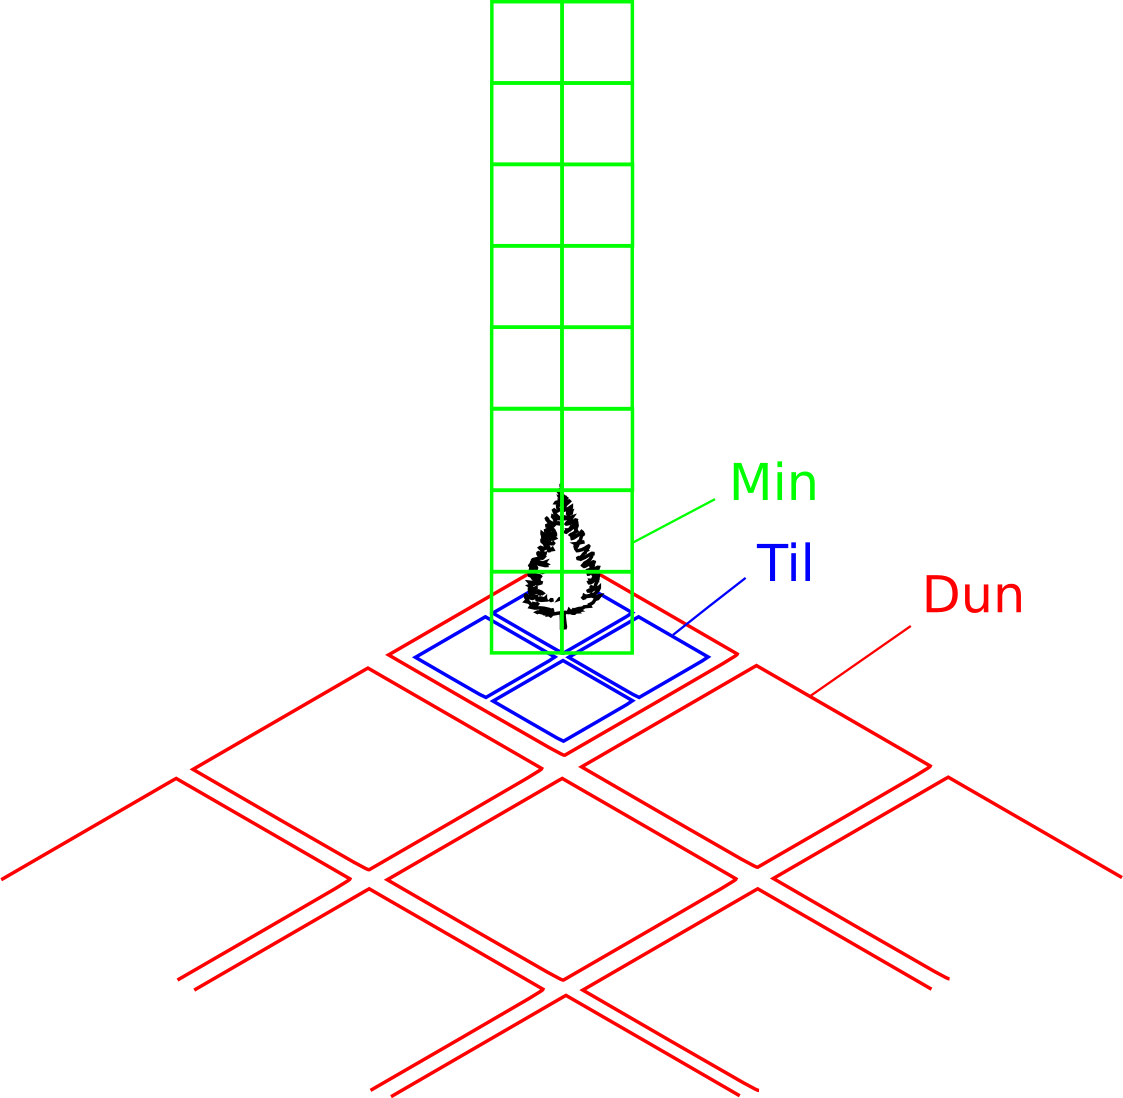
\includegraphics[scale=0.6]{level}\end{center}
    
    The properties of each tile is defined in the SOL file.

    \subsection{DUN files}
    DUN files are quite simple. They are essentyially a giant array of int16\_t s. The first two numbers are the width and height of the level (divided by four, as each block in the dun represents four actual level tiles). The remaining numbers are indices into the TIL file for each group of four tiles. Below is a c-style struct representing the structure of a dun file.
    \begin{lstlisting}
struct Dun
{
    int16_t width;
    int16_t height;
    int16_t blocks[width][height];
};
    \end{lstlisting}

    \subsection{TIL files}
    TIL files are also quite simple. they are just a massive array of int16\_t s, where each group of four is a block that can be referred to by the DUN file.

    \begin{lstlisting}
struct TilBlock
{
    int16_t top;
    int16_t left;
    int16_t right;
    int16_t bottom;
};

struct Til
{
    TilBlock blocks[FILESIZE/4];
};
    \end{lstlisting}

    \subsection{MIN files}
    MIN files are slightly awkward in that their size is not set. In l4.min and town.min, each entry is of size 16, but for all others they are 10.
    MIN files essentially are a list of blocks, recording the cel frame indices used for each. They are each a pillar with two images on each level, allowing a block to have things up above it (eg, a tree). They start at the top and work down, as illustrated in the image below:\\
    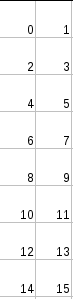
\includegraphics{minpillar}
    
    \subsection{SOL files}
    SOL files have not been fully figured out, however they are used becuase we can get some useful information out of them.
    Each byte in the SOL file is a bit field correcponding to an entry in the MIN file. Currently the only known value is the least signifigant bit, which indicates if a block is "passable" by the player and npcs (ie ground is passable, a wall isn't). A 0 in this position indicates that the block is passable, a 1 that it is not.
